\documentclass[../Lael_John_MasterThesis_Draft.tex]{subfiles}
\graphicspath{\subfix[../images]}
\begin{document}
The title of this thesis comes from an open question about tensors. Tensors are mathematical tools that are used to describe multiple linear relationships between mathematical objects. This ability of tensors to describe such inter-related information has spurred the study of \textit{multi}-linear algebra. The focus of this thesis is threefold: how are tensors constructed, where --- as mathematical objects --- do they live, and how they can be broken down? 

The current state of Comon's conjecture, an open problem for the past 20 years, is hard to describe succinctly. While mathematicians have steadily increased the number of cases for which the conjecture remains valid (highlighted at the end of \Cref{chapter:litreview}), an answer to the question in full generality for $\reals$- or $\complex$-tensors remains unknown.  The hope of this thesis is to provide a solid understanding of the work done in recent years, some of which may prove useful in constructing a counterexample to the conjecture, and to fill in the gaps present in the literature by giving formal definitions, lemmas, theorems and proofs where needed.
\begin{figure}
    \centering
    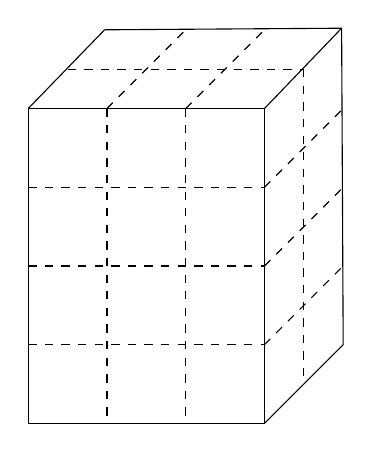
\begin{tikzpicture}[scale=1]
        % Coordinates
        \coordinate (A) at (1.00, 8.00);
        \coordinate (B) at (1.97, 9.00);
        \coordinate (C) at (4.00, 8.00);
        \coordinate (D) at (4.98, 9.02);
        \coordinate (E) at (4.00, 4.00);
        \coordinate (F) at (5.00, 5.00);
        \coordinate (G) at (1.50, 8.50);
        \coordinate (H) at (4.50, 8.50);
        \coordinate (I) at (4.50, 4.50);
        \coordinate (J) at (2.00, 8.00);
        \coordinate (K) at (2.00, 4.00);
        \coordinate (L) at (3.00, 8.00);
        \coordinate (M) at (3.00, 4.00);
        \coordinate (N) at (3.00, 9.00);
        \coordinate (O) at (4.00, 9.00);
        \coordinate (P) at (1.00, 7.00);
        \coordinate (Q) at (4.00, 7.00);
        \coordinate (R) at (5.00, 8.00);
        \coordinate (S) at (1.00, 6.00);
        \coordinate (T) at (4.00, 6.00);
        \coordinate (U) at (5.00, 7.00);
        \coordinate (V) at (1.00, 5.00);
        \coordinate (W) at (4.00, 5.00);
        \coordinate (X) at (5.00, 6.00);

        % Drawing
        \draw (1,4) rectangle (4,8);
        \draw (A) -- (B);
        \draw (C) -- (D);
        \draw (E) -- (F);
        \draw (B) -- (D);
        \draw (F) -- (D);
        \draw[dashed] (G) -- (H);
        \draw[dashed] (H) -- (I);
        \draw[dashed] (J) -- (K);
        \draw[dashed] (L) -- (M);
        \draw[dashed] (J) -- (N);
        \draw[dashed] (L) -- (O);
        \draw[dashed] (P) -- (Q);
        \draw[dashed] (Q) -- (R);
        \draw[dashed] (S) -- (T);
        \draw[dashed] (T) -- (U);
        \draw[dashed] (V) -- (W);
        \draw[dashed] (W) -- (X);
        \end{tikzpicture}
    \caption{Example of a tensor $T \in \field^4 \otimes \field^3 \otimes \field^2$, represented in the form of a $3$-way array}
\end{figure}

\nomenclature[A]{$\field$}{A general field, in this thesis either $\reals$ or $\complex$ unless specified}%
This question about symmetric tensors merits study because of the powerful nature of tensors as describing of multilinear relationships. One of the more important problems that has come to light in recent years is the computational complexity of matrix multiplication (\cite{landsberg_tensors_2012}), and tensors and their ranks help to quantify exactly how efficient the algorithms for matrix multiplication are. Tensors also find their use in quantum mechanics (describing the entanglement of particles), general relativity (as tools to describe the curvature of space-time \cite{carroll_spacetime_2019}), chemometrics and psychometrics (representing combinations of chemicals or traits that are interrelated \cite{zhang_comons_2016}), in data science and computer vision \cite{panagakis_tensor_2021} and in signal processing (the source selection problem \cite{landsberg_tensors_2012}) --- to name some more examples. 

% In each of these cases, the feature of problems being symmetric is seen as the more "natural" formulation of a problem, or the most elegant way of stating a problem. Knowing exactly how important symmetry is when describing such multilinear relationships is an important question, one that must be asked, even it it means sacrificing a more "beautiful" formulation for one that better reflects reality.
% % In each of these cases, knowing how important symmetry is as a feature of the relationship would play a vital role in analysing procedures and algorithms that take for granted that symmetry is the more "natural" state of affairs.
% This forms the guiding idea behind the ideas and techniques explored during this thesis.

\section*{Comon's Conjecture}\label{section:comonsconjecture}
At its heart, Comon's Conjecture centers around two central themes: the \textit{rank} and the \textit{symmetry} of tensors. A tensor's rank describes how it can be decomposed into much simpler constituent tensors, and its symmetry describes how the tensor behaves under permutation actions.

The conjecture was first stated openly in July 2008 at "Geometry and Representation Theory of Tensors for Computer Science, Statistics and Other Areas" - a workshop organised at the American Institute for Mathematics \cite{oeding_report_2008} in the group focusing on "Multilinear Techniques in Data Analysis and Signal Processing". The conjecture as stated in the report is as follows:

\begin{conjecture}[Comon \cite{oeding_report_2008}]
    Do the rank and symmetric rank of $T$ always coincide, where $T$ is a symmetric, real or complex tensor?
\end{conjecture}

This report also covered work done previously by Comon et al. \cite{comon_symmetric_2008} where they also showed that the conjecture held for conditions bounding the symmetric rank or order of a tensor in question. 
% when the symmetric rank of a tensor was at least as large as the dimension of the underlying vector space, or when the order (see \Cref{defn:tensororder}) of $T$ was sufficiently large
Since 2008, the mathematical community has further proved the conjecture true under various other assumptions. 

In 2018, Shitov \cite{shitov_counterexample_2018} proposed the construction of a counterexample living in $(\complex^{800})^{\otimes 3}$ with symmetric rank at least $904$, and a rank of at most $903$. In 2024 however, an erratum published (Draisma \cite{draisma_erratum_2024}) pointed out an error in the original paper, rendering the conjecture still unresolved in the complex case. In the intervening time, a paper published by Wang and Seigal \cite{wang_lower_2023} demonstrated the construction of a real, order-$6$, symmetric tensor having real rank $30913$ and symmetric rank $30914$, thus disproving the conjecture for the real case. Their paper built on a method of construction developed in a preprint from Shitov in 2020 \cite{shitov_comons_2020}. These ideas have also been developed further in subsequent preprints - \cite{shitov_higher_2024} and \cite{shitov_higher_2024-1}, again from Shitov.

\nomenclature[D]{$T^{\otimes d}$}{The tensor product of $T$ with itself $d$ times, $\underbrace{T \otimes T \otimes \cdots \otimes T}_{\text{$d$ times}}$}%

The following chapters and and subsequent sections highlight important terminology required to state and describe the setting of Comon's conjecture, review the work done to prove or disprove the conjecture in the past, and describe the major constructions required in the construction of the real counterexample.
\begin{description}
    \item[Chapter 2: Preliminaries Regarding Tensors] covers some preliminary terminology and definitions required to understand the history of attempts to prove Comon's conjecture. Personal contributions in this chapter include the proof of a theorem showing the isomorphism between symmetric tensors of fixed order and homogenous polynomials of fixed degree, \Cref{lemma:rankrelationshipwithonemode}, \Cref{defn:slicingoperator}, \Cref{defn:slicespace}, \Cref{defn:tensorunravelling} and \Cref{defn:flatteningoperator}. 
    \item[Chapter 3: Literature Review] reviews the literature that currently exists since the statement of the problem in 2008. The papers discussed highlight the valid attempts at proving Comon's conjecture over $\reals$ and $\complex$, and the attempts to construct a counterexample. Personal contributions to this chapter are the compilation of all these results in a singular location, highlighting the state of the art currently.
    \item[Chapter 4: Constructions Required for a Counterexample] focuses on understanding Shitov's methodology and approach to constructing a counterexample to Comon's conjecture. The culmination of this chapter is an examination of Wang and Seigal's publication \cite{wang_lower_2023}, which presents real-valued counterexample to the conjecture. Personal contributions to this chapter include explicit proofs for the various operations discussed, most of which do not exist in the existing literature. 
    \item[Chapter 5: Conclusion] illustrates problems with the current approach to constructing counterexamples and seeks to highlight potential future avenues to solving this problem once and for all. 
\end{description}
Further personal contributions to this thesis include all the illustrations and examples, used to shed light on definitions given through the entire document.
% The personal contributions made in the process of writing thesis are in the compilation of existing literature surrounding Comon's conjecture, establishing lemmas required for the constructions made by Shitov, and (wherever possible) either generalising  the arguments made by Wang and Seigal or showing why a generalisation is not possible. 
\end{document}